% !TEX encoding = UTF-8 Unicode
%!TEX root = ../Main/thesis.tex
% !TEX spellcheck = en-US
%%=========================================
\documentclass[../Main/thesis.tex]{subfiles}
\begin{document}
\chapter[Hilbert-Huang transform applied to bearing fault detection]{Hilbert-Huang transform for bearing fault detection}
\label{sec:hht}

Most signal decomposition methods such as Fourier transform, impose a-priory basis functions on the signal to be analyzed. In the case of Fourier analysis, the basis functions are trigonometric extensions. Although this implies a rigorous mathematical treatment, the resulting signal decomposition is limited by the mathematical assumptions (\cite{huang98}, \cite{huang08}). Limiting not in the sens of its mathematical truthfulness, rater in it ability to capture all intended salient physical properties of the target signal. Two such assumptions are linearity and stationary. As most phenomena in nature are nonlinear and non stationary, this mathematical approach, although rigorous, lacks an important property: Adaptivity (\cite{huang98}, \cite{huang08}). The latter refers to capturing the intrinsic properties of a signal, without imposing a-priory basis functions, (\cite{huang98}, \cite{huang08}). 
\justify 
The Hilbert-Huang transform (HHT) was precisely developed to deal with nonlinear and non stationary processes, in an adaptive fashion (\cite{huang98}). It combines Hilbert spectral analysis with the so call empirical mode decomposition (EMD), to adaptively decompose a signal into its fundamental components called intrinsic mode functions (IMF), (\cite{huang98}).
The richness of the HHT spans from the analysis of differential equations, to the study of geophysical phenomena, as well as bearings faults detection (\cite{huang08},\cite{li2009}, \cite{yan2006} ,\cite{soualhi2015}, \cite{sallo2019}), and by no mean limited to them.
\justify
 The HHT has been successful applied to the analysis of solutions of nonlinear differential equations, such as the Duffing and the Lorentz equations. The intrinsic frequency, the forcing function and the low intensity subharmonics of the numerical solutions for the nonlinear Duffing equation has been extracted through the EMD process, (\cite{huang98}).
 \justify
  The decomposition of the solutions of Lorentz equation, revealed \say{transient components with different frequencies and damping characteristics}, which agreed with previous studies, (\cite{huang98}). The HHT application to seismic waves propagation, identified high and low frequency seismic waves (\cite{vasudevan2000}). In particular, its decomposition of the seismic waves induced by the 1999 Taiwan earthquake, revealed that \say{the Fourier transform underestimated low frequency energy} (\cite{huang2001}). The Hilbert-Huang transform emerged as a general signal decomposition tool, and in theory can be applied to any signals.
\justify
In this chapter, a new method based on Hilbert-Huang transform (HHT) in part, is postulated and tested, with signals generated by diverse bearings mounted on a motor. The novel technique, couples the HHT with a robust seasonal trend decomposition method called STL, to detect bearing faults. STL stands for seasonal trend decomposition based on LOESS. In short, the STL decomposes a target signal into a trend and oscillatory components also called  seasonality. The trend is a monotone curve, while the seasonal components are periodic oscillations with constant period.
\justify
The bulk of the proposed scheme, consists of decomposing a target signal into (nearly) mono components signals also called intrinsic mode functions (IMFs). Furthermore, The seasonal trend of each IMF is extracted trough the seasonal trend decomposition based on LOESS. Moreover, the power spectral density of the resulting seasonal components are computed. The idea is that the resulting power spectral density, which is the energy distribution per frequency contribution, will encompass bearing failure if any.
\justify
After giving an esquisse of the new method, the remaining of this chapter is organized in the following manner:
 Section \ref{sec:emd} presents the empirical mode decomposition (EMD), which is the back bone of the Hilbert-Huang transform for decomposing a signal adaptively. Section \ref{sec:pulse}, through a concrete case study, demonstrates the efficiency of the novel approach. It begins with a gentile reminder of  bearing faults characteristics, followed by a description of the experimental setup, that generated the data for this case study. Afterwards, the seasonal trend decomposition based on LOESS (STL) is presented, followed by a schematic description of the new scheme. Finally, the results of the case study are explained. In closing, section \ref{sec:limitation} gives a short summary of this chapter.
\justify



 
 %%%%%%%%%%%%%%%%%%%%%%%%%%%%%%%%%%%%%%%%%%%%%%%%%%%%%%%%%%%%%%%%%%%%%%%%%%%%%%%%%%%%%%%%%%%%%%%%%%%%%%%%
 \section{The Hilbert-Huang transform}
 \label{sec:emd}
 The Hilbert-Huang transform is the amalgam of the empirical mode decomposition (EMD) and the Hilbert transform.
  The former decomposes a target signal into components having the same spectral characteristics, and identified as intrinsic mode functions (IMFs), while the latter enables the extension of a real valued signal to its complex counterpart. Together, the empirical mode decomposition and the Hilbert transform, form the basis for accurately (in the physical and mathematical sens), analyzing amplitude and frequency modulated signal (\cite{huang98}).
\justify
As will be shown subsequently, the empirical mode decomposition (EMD), can be (almost) interpreted as a filter bank. Here is why: The EMD can be regarded as a process that maps a target signal frequency range, to each intrinsic mode function (IMF). That is, higher frequency regions will correspond to IMFs with high frequency oscillation, while lower frequency regions will correspond to lower frequency IMFs. That is the definition of a filter bank. The empirical mode decomposition is iterative in nature.


\justify
 For a target signal $s(t)$, the goal is to obtained its $n$ fundamental parts (IMFs), denoted here by $s_{j}, j =1,\cdots,n$, through the empirical mode decomposition, such that
\begin{equation}\label{eq:emd-decomposition}
s(t) = \sum_{j=1}^{n}s_{j}(t) + r(t),
\end{equation}
where $r(t)$ is the residual, which is either a constant or a monotone function. The derivation of the intrinsic mode functions $s_{j}$, by means of the empirical mode decomposition, relies on the following key assumptions.
\begin{definition}\label{def:emd}
An intrinsic mode function (IMF) must satisfy the following conditions:
\begin{enumerate}
\item The number of extrema and the number of zero crossing must either equal or differ by one 
\item At any data point, the mean value of the envelope defined using the local maxima and the envelope defined by using the local minima is zero.
\end{enumerate}
\end{definition}
The empirical mode decomposition as an iterative algorithm, generates intrinsic mode functions, each satisfying definition \ref{def:emd} and obtained as follow:
\begin{enumerate}
	\item Compute the upper and the lower envelope curve of the target signal $s(t)$
	\item In the first iteration ($i=1$), compute the mean $m_{i}(t)$ between the upper and the lower envelope cure of $s(t)$
	\item Compute the first (pseudo) IMF as 
	\begin{equation}\label{eq:proto}
		h_{i1}(t) = s(t)-m_{i}(t).
	\end{equation}
	If $h_{i1}$ satisfies definition \ref{def:emd}, then it is an IMF and it is denoted by 
	\begin{equation}\label{eq:imf}
		c_{i}(t) = h_{i1}(t).
	\end{equation}
	otherwise
	
	\item Set $h_{i1}(t)$ as the input signal and repeat step 1,2 and 3, $k$ time, until $h_{ik}(t)$ satisfies definition \ref{def:emd}.
	\item After finding the first IMF, set the first IMF as input signal and repeat step 1,2,3 and 4 to obtain the remaining IMFs. If an IMF is monotone, set it as the residual and you are done.
\end{enumerate}
 In most function (signal) decomposition methods, a set of predefined $n$ basis functions denote here by $\varphi_{j}(t), j = 1,\cdots,n$, coupled with coefficients $a_{j}$, are used to decomposing a function, say $f(t)$ as 
\begin{equation}\label{eq:basis}
	f(t) = \sum_{j=1}^{n}a_{j}\varphi_{j}(t).
\end{equation}
However, the Hilbert-Huang transform decomposes $f(t)$ as 
\begin{equation}\label{eq:hht1}
f(t) = \sum_{j=1}^{n}c_{j}(t) + r(t).
\end{equation}
In equation (\ref{eq:basis}) the basis $\varphi_{j}(t)$ are chosen before hand (a-priory), and the coefficients are computed through an integral or summation operation. A kind of \say{bias} is imposed on the the function $f(t)$. A change of basis function will affect the resulting decomposition. On the other hand, in equation (\ref{eq:hht1}), the basis functions are directly derived from the properties of the function $f(t)$. This illustrates the concept of adaptivity, central to the Hilbert-Huang transform, which can be regarded as basis function agnostic.
\justify
Consider the signal
\begin{equation}
	s(t) = \sin(5 \pi t) + \sin(10 \pi t) + \sin(100 \pi t),
\end{equation}
  given in Figure \ref{fig:emd3}. It is made of one high frequency component (with angular frequency 100$\pi$) and two relatively low frequency components, with angular frequency 5$\pi$ and 10$\pi$, respectively. By applying the empirical mode decomposition, the three components are extracted and can be seen in Figure \ref{fig:signalimfs}. The first intrinsic mode function corresponds to the highest frequency component in the original signal (Figure \ref{fig:emd3}), while the second and third intrinsic mode functions correspond to the lower frequency components. This justifies the assertion made earlier, comparing the empirical mode decomposition to a filter bank. 
  \begin{figure}
   \centering
   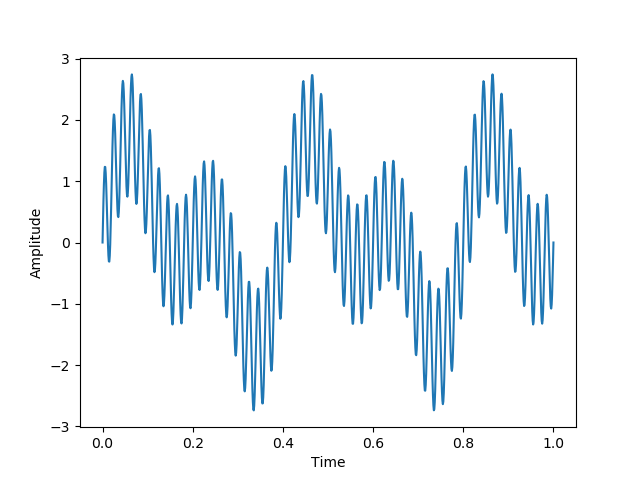
\includegraphics[width=6in]{../fig/sinusoidal.png} 
   \caption{ An input signal $s(t) = \sin(5 \pi t) + \sin(10 \pi t) +\sin(100 \pi t) $, with three frequency components}
   \label{fig:emd3}
\end{figure}

\begin{figure}[H]
	\centering
	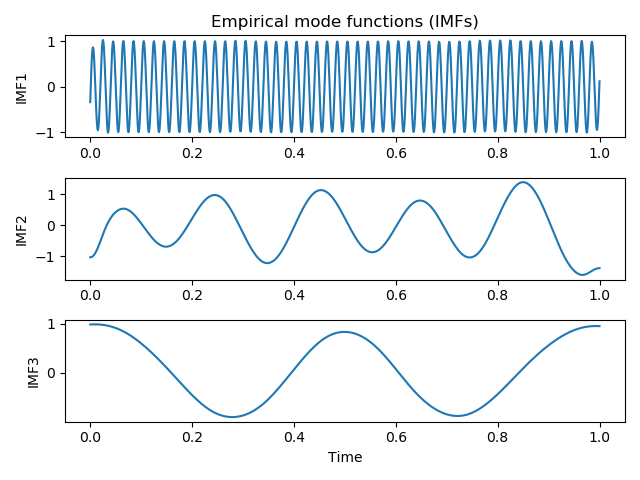
\includegraphics[width=0.8\linewidth]{../fig/signal_imfs}
	\caption{}
	\label{fig:signalimfs}
\end{figure}


\justify
The intrinsic mode functions obtained through the EMD process, constitutes an adaptive basis that satisfies the mathematical properties of convergence, completeness, orthogonality and uniqueness, (\cite{huang98}). Furthermore, if $a_{j}(t)$ and $\omega_{j}(t)$ are amplitude and frequency modulation corresponding to IMF $j$, then the original signal $s(t)$ can also be recovered as 
\begin{equation}\label{eq:recover2}
s(t) = \Re{\left( \sum_{j=1}^{n}a_{j}(t)\exp\left(i\int\omega_{j}(t)\mathrm{dt}\right)  \right)},
\end{equation} 
where the symbol $\Re(\cdot)$ represents the real part of the expression its encompasses, $i=\sqrt{-1}$, and $n$ is the total number of IMFs obtained from decomposing a signal $s(t)$. Recall that the amplitudes $a_{j}(t)$ and the frequencies $\omega_{j}(t)$ can be computed through the Hilbert transform. An analog representation of equation (\ref{eq:recover2}) in terms of Fourier expansion would be 
\begin{equation}\label{eq:recoverFourier}
s(t) = \Re{\left( \sum_{j=1}^{n}a_{j}\exp\left(i\omega_{j}\right)  \right)},
\end{equation} 
where this time, the amplitude $a_{j}$ and the frequency $\omega_{j}$ are constant. The Hilbert-Huang transform (HHT) offers two different approaches to recover a decomposed signal. The first one is described by equation (\ref{eq:hht1}) and includes the IMFs, while the second approach is given by equation (\ref{eq:recover2}) and includes the instantaneous amplitude and the instantaneous frequency. This gives the HHT a leverage over Fourier transform in nonlinear an non stationary data analysis.
\justify
The intrinsic mode functions resulting from the empirical mode decomposition, are not exactly mono components. That is, their spectral characteristics are not uniform in terms of their frequency content. This can be seen in Figure \ref{fig:imfsfreqband}, which displays the intrinsic mode functions of an input vibration signal, given in Figure \ref{fig:input}. The IMF number six (6), although representing a high frequency region of the original signal, displays bands of relatively low frequencies area. This mixture of high and low frequency regions, is called mode mixing.
\begin{figure}[H]
	\centering
	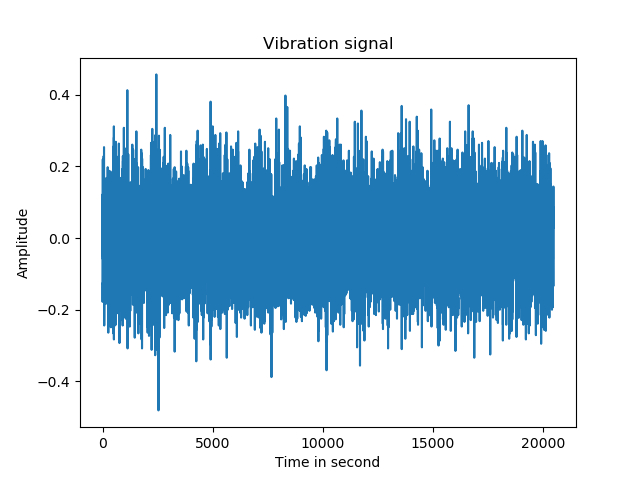
\includegraphics[width=0.8\linewidth]{../fig/input}
	\caption{An input vibration signal}
	\label{fig:input}
\end{figure}
\begin{figure}[H]
	\centering
	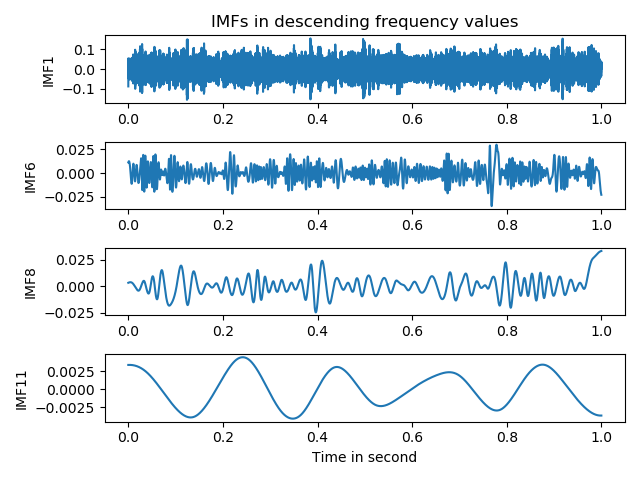
\includegraphics[width=0.9\linewidth]{../fig/imf_freq_band}
	\caption{Selected intrinsic mode function in descending frequency values.}
	\label{fig:imfsfreqband}
\end{figure}

%%%%%%%%%%%%%%%%%%%%%%%%%%%%%%%%%%%%%%%%%%%%%%%%%%%%%%%%%%%%%%%%%%%%%%%%%%%%%%%%%%%%%
%%%%%%%%%%%%%%%%%%%%%%%%%%%%%%%%%%%%%%%%%%%%%%%%%%%%%%%%%%%%%%%%%%%%%%%%%%%%%%%%%%%%%
%%%%%%%%%%%%%%%%%%%%%%%%%%%%%%%%%%%%%%%%%%%%%%%%%%%%%%%%%%%%%%%%%%%%%%%%%%%%%%%%%%%%%

\section{Application to bearing fault detection: a case study}
\label{sec:pulse}
In this section, the proposed new method is applied to a case study, in order to demonstrate its ability in detecting bearing failure. As a reminder, Figure \ref{fig:bearing-architecture} shows a geometry of a bearing, with different parts.
\begin{figure}[H] %  figure placement: here, top, bottom, or page
   \centering
   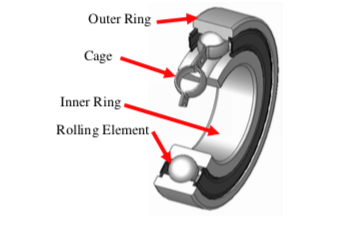
\includegraphics[width=4in]{../fig/bearing.png} 
   \caption{Geometrical representation of a bearing}
   \label{fig:bearing-architecture}
\end{figure}
\justify
A fault occurring in the outer ring is called a ball pass frequency outer ring (BPFO) defect, while a fault in the inner ring occurs at a frequency called ball pass inner race frequency (BPFI). Both are given in Hz in terms of the bearing geometrical characteristics an the rotating speed of the shaft as
\begin{equation}\label{eq:bpfo2}
BPFO = \frac{nb}{2}R\left(1-\frac{BD}{PD}\cos\left(\beta\right)  \right) \nonumber
\end{equation}
\begin{equation}\label{eq:bpfi2}
BPFI = \frac{nb}{2}R\left( 1 +  \frac{BD}{PD}\cos\left(\beta\right)   \right),
\end{equation}
where R is the rotating speed of the motor on which the bearing is attached. nb is the number of rolling elements (balls), BD is a rolling element diameter. The pitch diameter PD is half the height of the inner ring, and the contact angle $\beta$ is the angle formed when a rolling element touches the cage. 
\justify
The data and the experimental setup used for this case study were described in chapter 2. In this setup, four bearings are mounted on a motor rotating at 2000 rotations per minutes (33.3 Hz). In the first experiment the motor runs until
bearing number 3 is severely damaged with inner race defect, while in the second experiment outer race defect occurs in bearing number 1. For each experiment, successive vibration signals where obtained, with a sample rate of 20 $KHz$ and corresponding Nyquist frequency of 10 $KHz$ (half the sampling rate). The Nyquist frequency define a lower bound limit in order to avoid aliasing, which is a loss of information due to under sampling. That is, if the sample contain frequency components that are higher then the Nyquist frequency, those frequency components wont be able to be seen.

\justify
\subsection{Seasonal Trend decomposition based on Loess (STL)}
The STL sequentially applies the locally estimated scatter plot smoother (LOESS) in order to obtain cyclical and trend components of a signal (\cite{Cleveland-1979}, \cite{Cleveland-et-al-1988}). Here a cyclical component is a periodically occurring pattern in a signal. The  locally estimated scatter is a non parametric curve fitting procedure.  It can be used for \say{Data exploration, diagnostic checking of parametric models and provides a non parametric regression surface}.
If $s(t)$ is a signal, the goal is to obtained the decomposition 
\begin{equation}
s(t) = T_{r}(t) + C_{y}(t) + R_{res}(t),
\end{equation} 
where $T_{r}(t)$ an $C_{y}(t)$ are the trend and cyclical components, and $R_{res}(t)$ is the residual obtained from subtracting  the trend and the cyclical component from the signal. The key ingredient in the STL, is the locally estimated scatter plot smoother procedure. The latter being a non parametric regression method, does not rely on any a-priory assumption on the shape of the curve that needs to be fitted. It therefore provides a flexible approach to curve fitting, by capturing local, as well as global characteristics of a signal. A detailed account of the STL can be found in  (\cite{Cleveland-et-al-1990}).
\justify
 In this thesis, the STL is applied to address the mode mixing issue discussed earlier. This approach advantage is two folded: In one hand it solves the mode mixing issue by extracting the dominant frequency mode, and on the other hand
  its generates a clear frequency spectrum, as will be shown later.
%%%%%%%%%%%%%%%%%%%%%%%%%%%%%%%%%%%%%%%%%%%%%%%%%%%%%%%%%%%%%%%%%%%%%%%%%%%%%%%%%%%%%%%%%%%%%%
%%%%%%%%%%%%%%%%%%%%%%%%%%%%%%%%%%%%%%%%%%%%%%%%%%%%%%%%%%%%%%%%%%%%%%%%%%%%%%%%%%%%%%%%%%%%%%

\subsection{Results and interpretation}
In this section we apply the empirical mode decomposition followed by the seasonal trend decomposition based on LOESS to extract features containing bearings diagnostic information.
Figure \ref{fig:pulse} shows the flow diagram describing the new method for bearing fault detection.
\justify
An input bearing vibration signal is subjected to the empirical mode decomposition in order to generate intrinsic mode functions (IMFs). To mitigate mode mixing, the seasonal component of each IMF is extracted through the seasonal trend decomposition based on LOESS. In order to expose potential bearing failure frequencies, the power spectral density of the resulting signal is approximated by the periodogram method.
\justify
The power spectral density is technically the power or energy distribution of the autocovariance function (ACF) frequency spectrum. (\cite{stoica2004}). The autocovariance function of a signal $s(t)$ is defined by 
\begin{equation}
	ACF(s(t)) = E\left[ s^{*}(t)s(t-k) \right] = COV\left(s(t), s^{*}(t-k)\right)\quad k = 0,1, \cdots
\end{equation}
where $E(\cdot)$ is the expectation or mean, COV($\cdot$) is the covariance and $s^{*}(t)$ is the complex conjugate of $s(t)$. The covariance of the signal $s(t)$ and its complex conjugate measure their joint variability. Thus the autocovariance function is a sequence of covariance between the signal and its complex conjugate. Now, the power spectrum density (PSD) of a signal s(t) can be defined by (\cite{stoica2004})
\begin{equation}\label{eq:psd}
	PSD\left(s(t)\right) = E\left[ \frac{1}{N} \left\vert \sum_{t=1}^{N} s(t)e^{-i\omega t}\right\vert^{2}   \right]
\end{equation}
where $N$ is an integer, $i=\sqrt{-1}$, $E(\cdot)$ is the expected value, and $\omega$ is the angular frequency. The estimate $\widehat{PSD}$ of the power spectral density given by
\begin{equation}
		\widehat{PSD}\left(s(t)\right) =  \frac{1}{N} \left\vert \sum_{t=1}^{N} s(t)e^{-i\omega t}\right\vert^{2}
\end{equation}
is called the periodogram.
\begin{figure}[H]
\begin{tikzpicture}
  [node distance=.8cm,
  start chain=going below,]
     \node[punktchain, join] (intro) {\textcolor{blue}{Input signal}};
     \node[punktchain, join] (probf)      {\textcolor{violet}{EMD}};
     \node[punktchain, join] (investeringer)      {\textcolor{blue}{IMFs}};
     \node[punktchain, join] (perfekt) {\textcolor{violet}{STL}};
     \node[punktchain, join] (perfekt) {\textcolor{blue}{Pulse signal}};
     %\node[punktchain, join, ] (emperi) {Fast Fourier transform};
     % \node (asym) [punktchain ]  {Asymmetrisk information};
      \begin{scope}[start branch=venstre,
        %We need to redefine the join-style to have the -> turn out right
        every join/.style={->, thick, shorten <=1pt}, ]
        \node[punktchain, on chain=going left, join=by {->}] (risiko) {\textcolor{blue}{Power spactrum density}};
      \end{scope}
      \begin{scope}[start branch=hoejre,]
      %\node (finans) [punktchain, on chain=going right] {Det finansielle system};
    \end{scope}
    \end{tikzpicture}
  \caption{Schematic description of the new scheme for bearing fault detection.}
   \label{fig:pulse}
\end{figure}
   
\justify
Figure \ref{fig:emd-stl} shows an input vibration signal from a bearing with a defect, its fifth intrinsic mode function, and the resulting seasonal trend extracted through the STL.

\begin{figure}[H] %  figure placement: here, top, bottom, or page
   \centering
   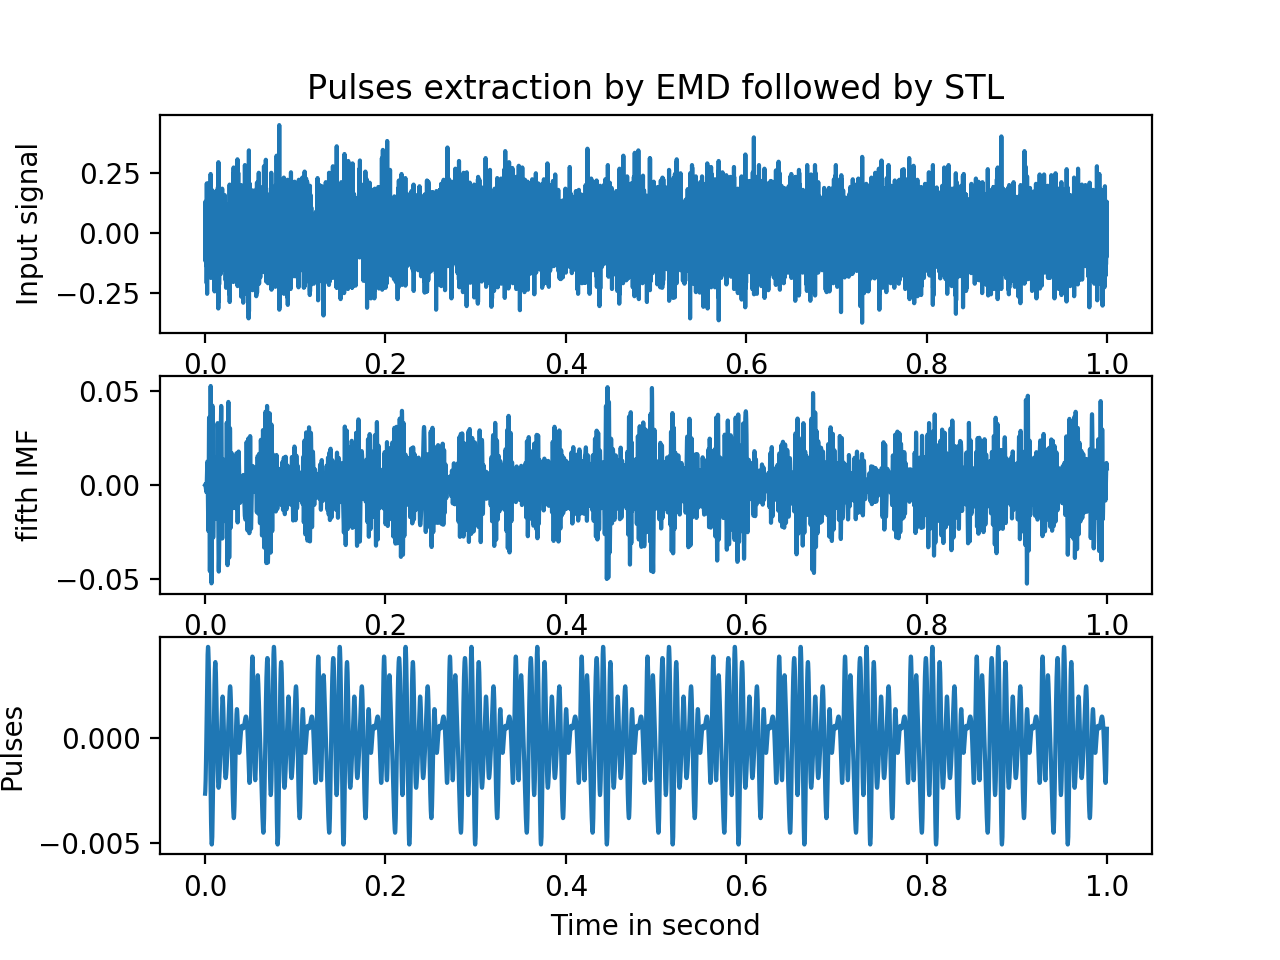
\includegraphics[width=6in]{../fig/emd-stl.png} 
   \caption{ A pulse signal extracted by applying EMD followed by STL. The top graph represents the vibration time signal. The middle graph is the fifth intrinsic mode function. The bottom graph is the signal resulting from applying the STL on the IMF. The pulses represents the periodic high frequency signal emitted by bearings defects.}
   \label{fig:emd-stl}
\end{figure}
\justify

The seasonal component of the intrinsic mode function has a pulse like shape (Figure  \ref{fig:emd-stl}, bottom graph). Here is why: As the bearing rotates, the roller elements (balls) strike the defect area, resulting in a sharp amplitude increase of the vibration signal. This process is repeated periodically through the machine operation. As will be shown shortly, this pulse signal contains all diagnostic information such as bearing failure frequencies, and their characteristics, the rotating speed of the machine, and other unidentified sources.
\justify
In the subsequent subsections, the power spectrum density of the seasonal component, from selected intrinsic mode function, is used to detect two types of bearing failure frequencies: Ball pass frequency outer race defect and ball pass inner race frequency defect. Recall that the power spectrum density is approximated here by the periodogram method.
\subsubsection{Ball pass outer race frequency defect detection} 
 \begin{figure}[H]
 	\centering
 	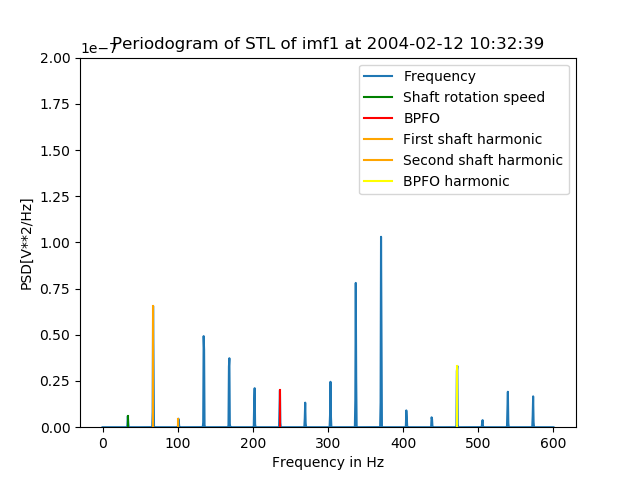
\includegraphics[width=0.8\linewidth]{../fig/periodogram_bpfo/start_imf1_bpfo}
 	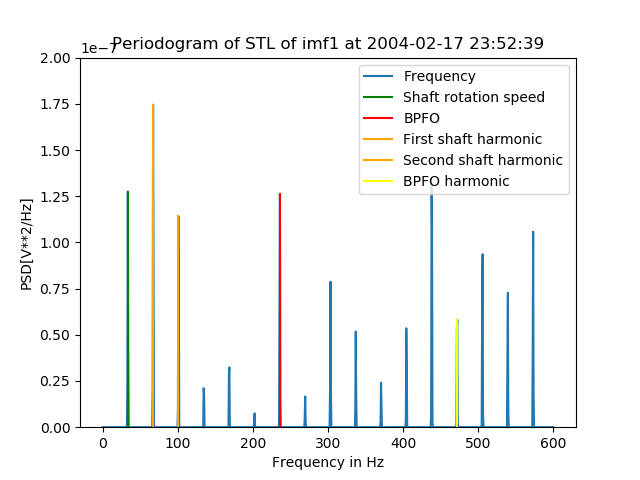
\includegraphics[width=0.8\linewidth]{../fig/periodogram_bpfo/end_imf1_bpfo}
 	\caption{Periodogram of the pulse signal obtained from the first IMF, at the beginning (top) and the end (bottom) of experiment number 2}
 	\label{fig:startimf1bpfo}
 \end{figure}
\justify
Figure \ref{fig:startimf1bpfo} shows the periodogram of the seasonal component from the first IMF obtained at the beginning (top) and at the end of experiment number 2. The periodogram shows conspicuous frequency peaks from 0 to 600 Hz approximately. At the beginning of the experiment, the ball pass outer race frequency defect (236.4 Hz) is visible with a relatively low amplitude. At the end of the experiment however, there is a relatively high increase in the outer race frequency defect amplitude, which exhibits the severity of the damage incurred by the bearing.
\justify
In addition, the rotating speed (33.3Hz) of the machine shaft is visible in both cases. Harmonics of the defect frequency are also visible. And the magnitude of the harmonics have also increased, as the bearing defect is accentuated. Recall that harmonics are characteristics of bearing outer race defect, and are integer multiple of the defect frequency (236.4 Hz) and machine speed (33.3 Hz). In bearing vibration analysis, harmonics are the tail tail sign of a ball pass outer race defect. The rest of the peaks in the periodogram represent unexplained phenomenon. Possibly signals from other part of the machine.
\justify
The difference between the theoretical value of the ball pass outer frequency defect (236.4 Hz) and the one from the periodogram (236.03 Hz) is about 0.16$\%$. While the difference between the theoretical shaft frequency (33.33 Hz) and the on the periodogram (33.63 Hz) is about 0.9 $\%$. This shows that the proposed method is relatively efficient in detecting important diagnostic information from the vibration signal. 
\justify
As pointed out earlier, the empirical mode decomposition, maps each intrinsic mode function to region of high and low frequencies in the original signal. As such we would expect low frequency processes such as the rotation speed of the machine, in the periodogram of lower frequency intrinsic mode functions. Figure \ref{fig:endimf8shaft} shows the periodogram of a lower frequency intrinsic mode function (IMF8). This IMF displays only a peaks corresponding to the rotation speed of the machine (33.3 Hz).
\begin{figure}[H]
	\centering
	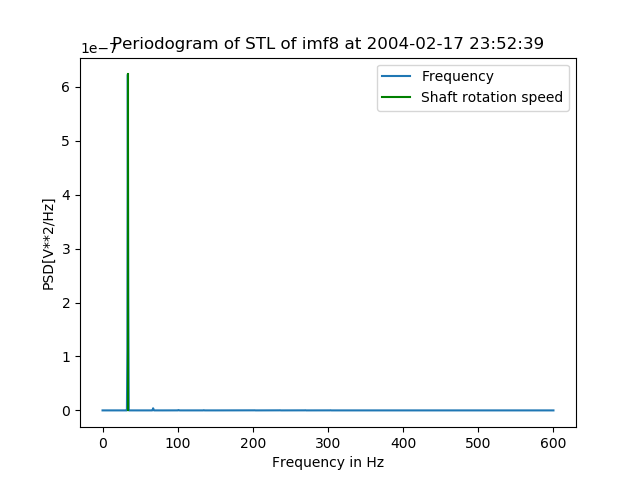
\includegraphics[width=0.9\linewidth]{../fig/periodogram_bpfo/end_imf8_shaft}
	\caption{Periodogram of a lower frequency intrinsic mode function, displaying a peak corresponding to the rotation speed of the machine housing the bearing}
	\label{fig:endimf8shaft}
\end{figure}


\subsubsection{ Ball pass inner race frequency defect detection }

\begin{figure}[H]
	\centering
	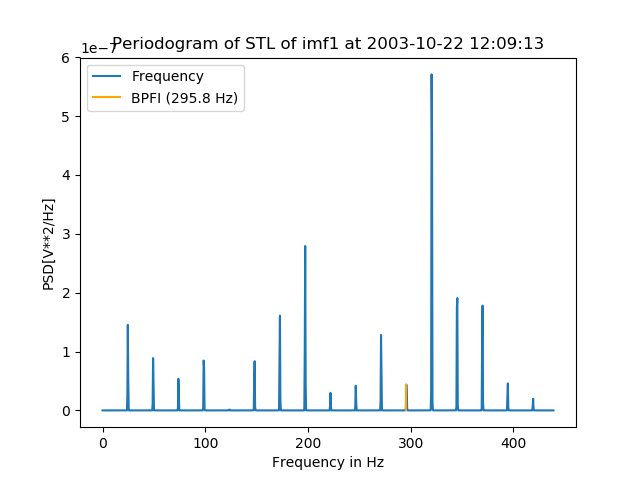
\includegraphics[width=0.8\linewidth]{../fig/periodogram_bpfi/start_imf1_bpfi}
	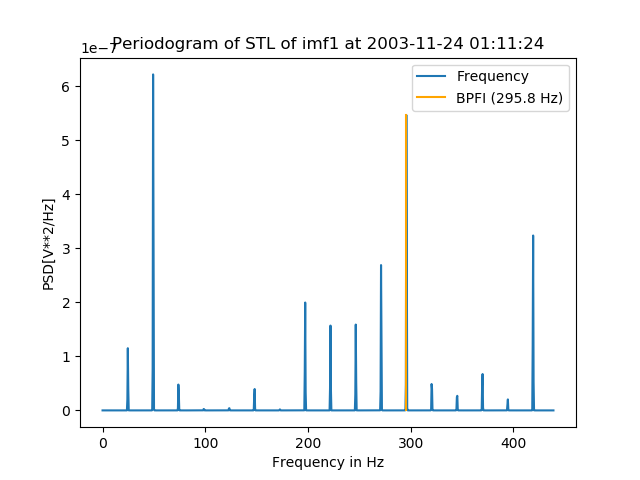
\includegraphics[width=0.8\linewidth]{../fig/periodogram_bpfi/end_imf1_bpfi}
	\caption{Periodogram of the pulse signal obtained from IMF number 1, at the beginning (top) and the end (bottom) of experiment number 1.}
	\label{fig:startimf1bpfi}
\end{figure}
\justify
Figure \ref{fig:startimf1bpfi} shows the periodogram obtained from the seasonal component of the first intrinsic mode functions at the start (top) and at the end (bottom) of experiment number 1. The inner race defect frequency (296.8 Hz) is visible in both cases.
However, the rotating speed of the machine (33.3 Hz) is not visible. The amplitude of the inner race defect frequency had increased considerably towards the end of the experiment. This again indicates that the defect incurred by the bearing had increased in severity.
The difference between the theoretical value of the BPFI (296.8 Hz) and the detected value (295.8) is about 0.33 $\%$. The periodogram also exhibits other frequency peaks for which we can not account for, due to lack of additional information.
\justify
\section{Summary}
\label{sec:limitation}
In this chapter, a new method for bearing fault detection was presented. This new technique uses the empirical mode decomposition (EMD), the seasonal trend decomposition based on LOESS, and the power spectrum density in order to identify bearing failure. The empirical mode decomposition splits an input vibration signal into components called intrinsic mode functions (IMFs). The first few IMFs contain high and low frequency components of the input signal, while the remaining IMFs contain mainly low frequency components of the input signal.
\justify
Once the IMFs are obtained, depending on the frequency range of the bearing failure frequencies, an IMF is chosen. In this thesis, the first IMF is chosen for bearing failure detection. Furthermore, the seasonal trend of the selected IMF is extracted, and the power spectrum density of the latter is approximated. By extracting the seasonal trend of the selected IMF, the mode mixing phenomenon incurred by the EMD is mitigated. Recall that mode mixing is the mixture of high and low frequency mode in an IMF. When mode mixing occurs, the generated IMF looses it physical meaningful property. 
\justify
The results from the proposed new method applied to a concrete case study, show that the new scheme is able to detect bearing failure, as well as their characteristics such as harmonics. In addition, lower amplitude intrinsic mode functions identify lower process such the rotation speed of the machine.
\justify


%The proposed method consists of transforming a vibration signal to a pulse like signal, which contains all diagnostics information in terms of bearing failure detection. In particular, the outer race and the inner race defect. The present method uses the empirical mode decomposition (EMD), followed by the seasonal trend decomposition method based on Loess (STL). The former is a signal decomposition method suited for non stationary and non linear signal, while the letter extracts periodic components from a signal.
%\justify
%Together they are able to generate a noise less periodogram which contains relevant frequency information for bearing fault detection. The periodogram approximates the power spectral density (PSD) of a signal. The PSD is the energy distribution of frequencies components of a signal.
%By applying the proposed method, it was possible to identify conspicuous outer and inner race defect frequencies, as well as the roation frequency of the machine shaft, in a periodogram pertaining to a bearing undergoing failure.








\blankpage
\end{document}

